% ============================================================
% DROP-IN REPLACEMENT for Draft_5c.tex lines 771-905
% (\subsection{Estimator Accuracy} ... "as wrong as it is right.")
%
% Keeps labels : sec:sensitivity, eq:meas_noise, eq:pos_noise,
%                fig:est_accuracy
% New labels   : eq:sigma_eff, eq:gain_ladder, eq:groups,
%                eq:error_budget, tab:budget
% Retired      : lem:gains, eq:gain_grad, eq:gain_hess, rem:eigvec, M_3
%                (see diffs D2, D3, D7, D8)
% ============================================================

\subsection{Estimator Sensitivity}
\label{sec:sensitivity}

Two channels perturb the samples. Measurement noise is additive
Gaussian on the components each robot reads,
\begin{equation}
    u_i^m = u(\mathbf{p}_i) + \eta_i^u, \quad
    v_i^m = v(\mathbf{p}_i) + \eta_i^v,
    \quad \eta \sim \mathcal{N}(0, \sigma_{uv}^2),
    \label{eq:meas_noise}
\end{equation}
independent across robots, components, and steps, the sensor model of
\cite{9}. Position noise perturbs where each robot
samples,
\begin{equation}
    (u_i^m, v_i^m) = \mathbf{v}(\mathbf{p}_i + \boldsymbol{\xi}_i), \quad
    \boldsymbol{\xi}_i \sim \mathcal{N}(\mathbf{0}, \sigma_p^2 \mathbf{I}),
    \label{eq:pos_noise}
\end{equation}
while the fit (\ref{eq:solve}) uses the nominal $\mathbf{p}_i$. A
displaced robot commits the reading error
$\mathbf{J}\boldsymbol{\xi}_i$ to first order, so the two channels
combine into one effective level,
\begin{equation}
    \sigma_{\mathrm{eff}}^2 = \sigma_{uv}^2
        + \tfrac{1}{2}\lVert\mathbf{J}\rVert_F^2\,\sigma_p^2 .
    \label{eq:sigma_eff}
\end{equation}

The fit is linear, so $\hat{\boldsymbol{\theta}} -
\boldsymbol{\theta} = \boldsymbol{\Phi}^{-1}\boldsymbol{\eta}$ exactly
and the analysis is a calculation of row norms. For the
pentagon-plus-center, a coefficient of derivative order $q$ has
\begin{equation}
    \sigma_{\theta_q} = \gamma_q\,
    \frac{\sigma_{\mathrm{eff}}}{\rho^{\,q}},
    \qquad
    \gamma_0 = 1, \;\;
    \gamma_1 = \tfrac{2}{\sqrt{10}}, \;\;
    \gamma_2 = \tfrac{8}{\sqrt{10}},
    \label{eq:gain_ladder}
\end{equation}
with $\gamma_2 = 4/\sqrt{10}$ for the mixed coefficients and gradient
covariance $\tfrac{4}{10}\sigma_{\mathrm{eff}}^2\rho^{-2}\mathbf{I}$,
isotropic at every heading (Appendix~\ref{app:proofs}). Only $\gamma_q$ is specific to this
formation; the exponent is not, since order $q$ costs $q$ difference
quotients and only the signal scales with $\rho$. An affine fit returns
no second derivatives at all: three robots locate a critical point
\cite{14}, six supply the curvature and eigenframe the trackers
consume.

Truncation pulls the other way. With $U$ and $L$ the velocity and length
scales of the field, form
\begin{equation}
    \nu = \frac{\sigma_{\mathrm{eff}}}{U}, \qquad
    \tilde{\rho} = \frac{\rho}{L}.
    \label{eq:groups}
\end{equation}
A quantity of order $q$ has magnitude $U/L^{\,q}$, so its relative noise
error is $\nu/\tilde{\rho}^{\,q}$, while the discarded term of order
$p+1$ biases it by a relative $\tilde{\rho}^{\,p+1-q}$:
\begin{equation}
    E_q(\tilde{\rho}) = c\,\frac{\nu}{\tilde{\rho}^{\,q}}
        + d\,\tilde{\rho}^{\,p+1-q}.
    \label{eq:error_budget}
\end{equation}
The exponents sum to $p+1$ by construction, noise counting the orders
extracted and truncation the orders remaining, so $\tilde{\rho}^*
\propto \nu^{1/(p+1)}$, a cube root here. The optimum differs between
$\hat{D}$ and $\nabla\hat{D}$, and neither constant is computable in the
field: $\rho$ is fixed at $0.075$ on the double gyre and set by the sampling requirement of
Section~\mbox{V-C} on the ocean field.

Two terms escape (\ref{eq:error_budget}), each adding a constant. Some
quantities need derivatives the model does not carry:
(\ref{eq:Dxx_true}) splits into a fitted pair and four third-order terms
of the same size as $D_{xx}$ itself, set to zero by construction rather
than made small by a good fit, contributing a floor $e = O(1)$
independent of $\rho$, $\sigma_{\mathrm{eff}}$, and formation.
The same audit of $\nabla D$ returns nothing, every term of it pairing a
fitted second derivative with a fitted first, so any measured gap
between the two is $e$ alone. The floor destroys sign information where
an eigenvalue crosses zero but leaves directions usable, so
$\hat{\mathbf{H}}_D$ can steer a controller and cannot tell it when to
stop. The second constant
is the observer: a rotation at $\Omega$ is absorbed by the spin part and
not the strain part, so (\ref{eq:D_not_objective}) contaminates every
determinant-derived quantity by a relative $O(\mathrm{Ro})$,
$\mathrm{Ro} = \Omega L/U$, again with no $\nu$, $\tilde{\rho}$, or
formation geometry in it.

Both surrogates sit on the same rung, and what separates them is
algebraic. $D$ is a quadratic form in the first-order coefficients,
while $s_1 = \mu - r$ is a norm subtracted from an affine function. A
perturbed norm projects the noise onto a unit vector, so $\sigma_{s_1} =
\gamma_1\sigma_{\mathrm{eff}}/\rho$ however poorly the eigenframe is
resolved; the eigenframe divides by that magnitude instead, and its
angular error carries an extra $1/r$.

\begin{table}[!t]
\centering
\caption{Error budget by channel. $\nu$ and $\tilde{\rho}$ are the
relative noise and radius of (\ref{eq:groups}), $e$ the
unmodelled-derivative floor, $\mathrm{Ro}$ the observer term, and $r$
the deviatoric strain magnitude of Section~\mbox{III-C}.
$\hat{\mathbf{H}}_D$ is at once the only curvature available to either
tracker and the only quantity either consumes that carries a floor.}
\label{tab:budget}
\footnotesize
\setlength{\tabcolsep}{4pt}
\begin{tabular}{@{}lccccc@{}}
\hline
quantity & noise & trunc. & floor & frame & gap \\
\hline
$\hat{D}$ & $\nu/\tilde{\rho}$ & $\tilde{\rho}^2$ & --- & $O(\mathrm{Ro})$ & --- \\
$\hat{s}_1$ & $\nu/\tilde{\rho}$ & $\tilde{\rho}^2$ & --- & --- & --- \\
$\nabla\hat{D}$ & $\nu/\tilde{\rho}^2$ & $\tilde{\rho}$ & --- & $O(\mathrm{Ro})$ & --- \\
$\nabla\hat{s}_1$ & $\nu/\tilde{\rho}^2$ & $\tilde{\rho}$ & --- & --- & --- \\
$\hat{\mathbf{H}}_D$ eigenvalues & $\nu/\tilde{\rho}^2$ & $\tilde{\rho}$ & $e = O(1)$ & $O(\mathrm{Ro})$ & --- \\
strain eigenframe & $\nu/\tilde{\rho}$ & $\tilde{\rho}^2$ & --- & --- & $\div\,r$ \\
$\hat{\mathbf{H}}_{s_1}$ & --- & --- & sign wrong & --- & undef. at $r=0$ \\
\hline
\end{tabular}
\end{table}

\begin{figure}[!t]
    \centering
    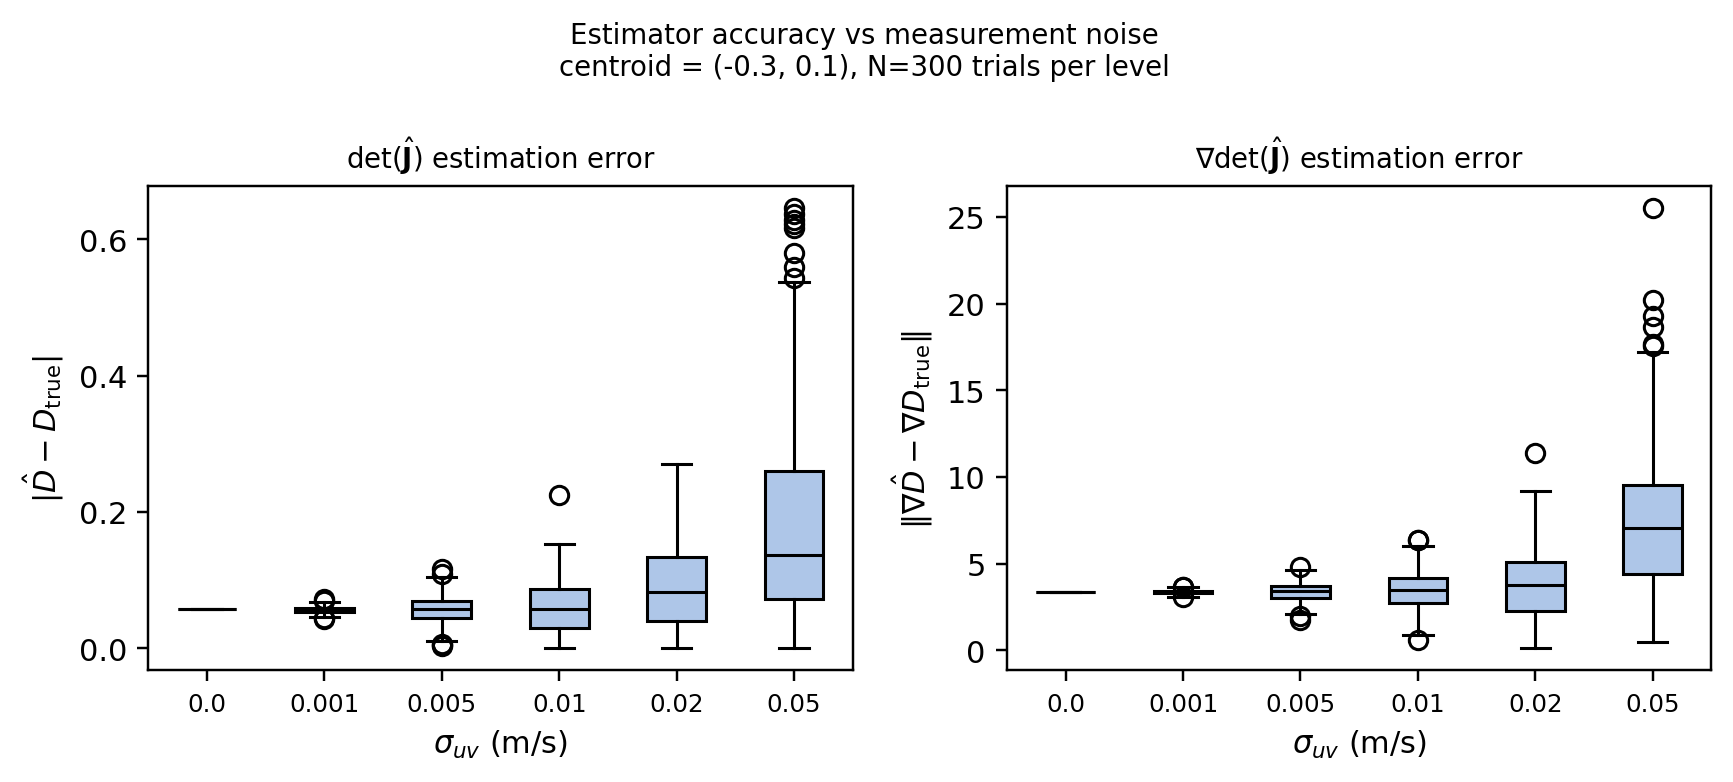
\includegraphics[width=0.34\textwidth]{figures/estimator_accuracy_vs_noise.png}
    \caption{Relative estimation error of $\hat{D}$, $\nabla\hat{D}$, and
    $\hat{\mathbf{H}}_D$ on the steady double gyre (median over $2 \times
    10^5$ noise draws per point; the dashed line marks error equal to
    signal). (a) Versus measurement noise at $\rho = 0.075$; the
    dash-dotted line marks the noise level where closed-loop traverse
    success crosses 50\% (Table~\ref{tab:mc_success}). (b) Versus
    formation radius at $\sigma_{uv} = 0.01$; dotted curves are the
    noise-free truncation floors. On these axes the exponents of
    (\ref{eq:error_budget}) appear as slopes.}
    \label{fig:est_accuracy}
\end{figure}

Over $2\times10^5$ draws per condition at a static strain-region point
of the double gyre, every coefficient standard deviation matched (\ref{eq:gain_ladder}) within 0.3\% and the position-noise
reading error matched (\ref{eq:sigma_eff}) within 1.1\%. In
Fig.~\ref{fig:est_accuracy}(a), $\hat{D}$ stays informative to
$\sigma_{uv} \approx 0.06$ and $\nabla\hat{D}$ to $\approx 0.01$, while
$\hat{\mathbf{H}}_D$ sits at the error-equals-signal line even for the
quietest sensors, held there by $e$; its eigendirections remain accurate
to $0.35^\circ$ near the separatrix and $3.8^\circ$ at a generic point,
the eigenvalues absorbing the floor. Closed-loop
degradation should therefore begin near $\sigma_{uv} = 0.01$.
